\section{Dead reckoning}
The accuracy of the representation of the players as well as the ball is important for the game to function well.
Since these positions are sent over the network, they might not always be the most recent positions, since they could be delay or packages lost.
\\\\
Dead reckoning is a technique that is used to predict where a game object is at current time based on its last know position, velocity and acceleration.
It is often used for networking games where packages about the object's kinematic state are continuously being sent from the server to the clients.
The kinematic state of an object includes its position, velocity, acceleration, orientation and angular velocity \autocite{DeadReckoning}.
If the client misses a package or they are not being sent often enough to have a new update for each frame, the representation of the object will jerk across the screen instead of having smooth and consistent movement.
That is where dead reckoning can be used to predict an objects movement to make it appear more believeable.
For the game we're building, it is important that each player's and the ball's positions are very accurate for the game to function properly.
\\\\
It is not possible have a new update for each frame, zero packet losses or zero latency. 
Therefore dead reckoning is needed to achieve a believeable representation of the ball and the players' movement \autocite{DeadReckoning}.
\begin{figure}[H]
    \centering
    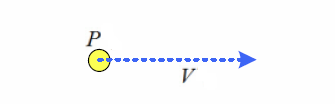
\includegraphics[width=0.6\linewidth]{dead_reckoning/dead_reckoning_example_1.PNG}
    \caption{Linear player movement}
    \label{fig:dead_reckoning_example_1}
\end{figure}
\autoref{fig:dead_reckoning_example_1} shows an example of a player's movement in the game.
In this example, dead reckoning would be a linear problem where the position, velocity and acceleration can be used to predict where the player will move to in the future. 
The dead reckoned position for a specific time $Q_t$ in this example can be calculated by:
\begin{displaymath}
    Q_t = P'_0 + V'_0T + \frac{1}{2}A'_0T^2
\end{displaymath}
where $ P'_0 $ is the position, $ V'_0 $ is the velocity, $ A'_0 $ is the acceleration and $T$ is the time \autocite{DeadReckoning}.
\begin{figure}[H]
    \centering
    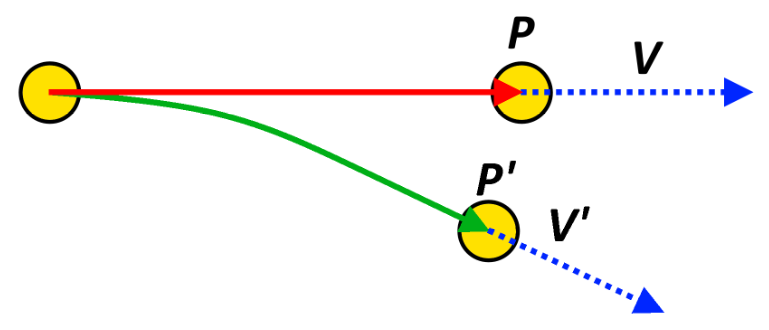
\includegraphics[width=0.6\linewidth]{dead_reckoning/dead_reckoning_example_2.PNG}
    \caption{A new update about the player's state is received from the server}
    \label{fig:dead_reckoning_example_2}
\end{figure}
In \autoref{fig:dead_reckoning_example_2} we receive a new update about the player's kinematic state. 
This results in conflicting realities when compared to the dead reckoned position calculated from the previous example. 
In the new update the player has turned right and a new dead reckoned position must be found, but this time it becomes a lot trickier since a believeable curve must be created from where we thought the player would be and where we estimate the player will be based on the new information. Representing the new position $P'_0$ immediately would result in the player warping across the screen which would not be ideal. Instead the player is represented at $ P_0 $ where we thought the player would be and the player should then move towards a new dead reckoned position, calculated with the information from the new update \autocite{DeadReckoning}.


\subsection{Projective Velocity Blending}
To calculate the curve that the player's movement needs to follow we need a good algorithm that is not too CPU intensive.
The algorithm must work well for a segment of a curve that is passing through two points being the player's current position $P_0$ and the estimated future location $P'_1$.
The recommened approach for this problem is projective velocity blending \autocite{DeadReckoning}.
\\\\
We create projections for the current kinematic state and the last known kinematic state and then these are blended together. 
\begin{displaymath}
    P_t = P_0 + V_0T_t + \frac{1}{2}A'_0T_t^2 \quad \rlap{\text{(Projecting from where player was)}}
\end{displaymath}
\begin{displaymath}
    P'_t = P'_0 + V'_0T_t + \frac{1}{2}A'_0T_t^2 \quad \rlap{\text{(Projecting from last known)}}
\end{displaymath}
\begin{displaymath}
    Q_t = P_t + (P'_t - P_t)\hat{T} \qquad \rlap{\text{(Combination of the two)}}
\end{displaymath}
\\\\
From this we get the dead reckoned location $ Q_t $ at the specified time. 
The reason that $ A'_0 $ is used in both projections is that it will converge to the player's true path much faster and it reduces oscillation, compared to when using $ A_0 $ when calculating $ P_t $. 
However, these calculations will still give inadequate results since the player's movement will have bad oscillations. 
These are cause by the changes in velocity,$V_0$ and $V'_0$, when new updates are received from the server. To account for this, a linear interpolation between the old velocity and the last known velocity is computed, which creates a blended velocity $V_b$. 
This velocity is used in the projection from where the player was, when a new update is received. 
This is what is known as \textit{projective velocity blending} \autocite{DeadReckoning}.
\\\\
\begin{displaymath}
    V_b = V_0 + (V'_0 - V_0)\hat{T} \quad \rlap{\text{(Velocity blending)}}
\end{displaymath}
\begin{displaymath}
    P_t = P_0 + V_bT_t + \frac{1}{2}A'_0T_t^2 \quad \rlap{\text{(Projecting from where player was)}}
\end{displaymath}
\begin{displaymath}
    P'_t = P'_0 + V'_0T_t + \frac{1}{2}A'_0T_t^2 \quad \rlap{\text{(Projecting from last known)}}
\end{displaymath}
\begin{displaymath}
    Q_t = P_t + (P'_t - P_t)\hat{T} \qquad \rlap{\text{(Combination of the two)}}
\end{displaymath}
This should reduce the oscillations in the player's movement significantly.
\begin{figure}[H]
    \centering
    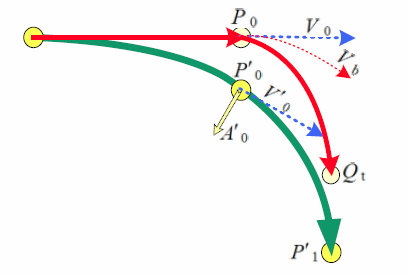
\includegraphics[width=0.6\linewidth]{dead_reckoning/dead_reckoning_example_3.PNG}
    \caption{Shows the the curve for the dead reckoned position $Q_t$ when making use of projective velocity blending}
    \label{fig:dead_reckoning_example_3}
\end{figure}
In \autoref{fig:dead_reckoning_example_3} we see the red curve that the player should follow to reach the dead reckoned position $Q_t$. $ P_0 $ is where we currently represent the player. $ P'_0 $ is the recent position received from the server. The green curve is the one that the player actually follows.
\\\\
This technique would be ideal to implement in the game if we find that the representation of the players' movement is inconsistent and in need of improvement.